\documentclass[../main.tex]{subfiles}

\begin{document}
	\subsection{Decentered Inverter}
	{
		\begin{tcolorbox}[colback=gray!5!white,colframe=gray!75!black]
			Plot the transfer function for a decentered inverter with
			\begin{itemize}
				\item $W_n = W_p = 3,0\mu m$
				\item $W_p = 12,0\mu m$ and $W_n = 3,0\mu m$
			\end{itemize}
			Deduce the noise margins on the input low state and high state.
		\end{tcolorbox}
		
		For a lower value of $W_p$, the PMOS transistor has a smaller $g_m = \frac{\partial I_D}{\partial V_{SG}} = k_p \frac{W}{L}(V_{SG} - |V_{tp}|)$. Thus, the PMOS is less sensitive to variations in $V_{SG}$ which makes the high-low transition slower. We expect $NML < NMH$.
		
		\begin{figure}[H]
			\centering
			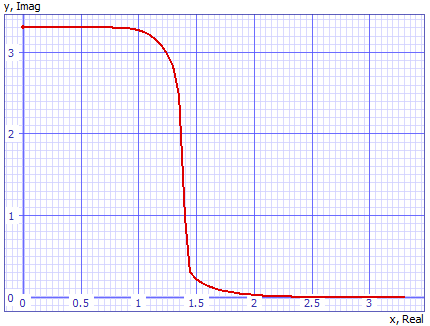
\includegraphics[width=0.5\textwidth]{plots/Q4_1.png}
			\caption{Transfer function for decentered inverter with $W_n = W_p = 3,0\mu m$}
		\end{figure}
		
		We get from the graphic
		
		\begin{itemize}
			\item $V_{IL} = 0,85$V (maximum $V_{in}$ for which $V_{out}$ is high)
			\item $V_{IH} = 2,22$V (minimum $V_{in}$ for which $V_{out}$ is low)
			\item again we consider $V_{OL} = 0$V and $V_{OH} = 3,3$V.
		\end{itemize}
		
		We conclude that
		\begin{itemize}
			\item $NML = V_{IL} - V_{OL} = 0,85$V
			\item $NMH = V_{OH} - V_{IH} = 3,3 - 2,22 = 1,08$V
		\end{itemize}
		
		Now for a higher value of $W_p$, the PMOS transistor has a higher $g_m = \frac{\partial I_D}{\partial V_{SG}} = k_p \frac{W}{L}(V_{SG} - |V_{tp}|)$. Thus, the PMOS is more sensitive to variations in $V_{SG}$ which makes the high-low transition faster.  We expect $NML > NMH$.
		
		\begin{figure}[H]
			\centering
			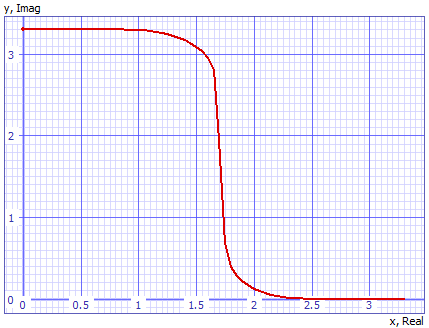
\includegraphics[width=0.5\textwidth]{plots/Q4_2.png}
			\caption{Transfer function for decentered inverter with $W_p = 12,0\mu m$ and $W_n = 3,0\mu m$}
		\end{figure}
		
		We get from the graphic
		
		\begin{itemize}
			\item $V_{IL} = 0,99$V (maximum $V_{in}$ for which $V_{out}$ is high)
			\item $V_{IH} = 2,35$V (minimum $V_{in}$ for which $V_{out}$ is low)
			\item again we consider $V_{OL} = 0$V and $V_{OH} = 3,3$V.
		\end{itemize}
		
		We conclude that
		\begin{itemize}
			\item $NML = V_{IL} - V_{OL} = 0,99$V
			\item $NMH = V_{OH} - V_{IH} = 3,3 - 2,35 = 0,95$V
		\end{itemize}
	
	}
\end{document}